% Chapter 2

\chapter{Water Balance} % Chapter title

\label{ch:WaterBalance} % For referencing the chapter elsewhere, use \autoref{ch:examples} 

%----------------------------------------------------------------------------------------
In the study of hydrology, the water influx and efflux of a system can be described using \textbf{Water Balance Model}. The system can be one of various domains and scales, such as a drainage basin across a large surface area\citep{Kirby2008}, or as small as the soil water balance in the root zone of a single plant\citep{Zhang2002}. For a soil-based water system, the influx of water includes precipitation and irrigation whilst the efflux of water includes surface runoff, subsurface runoff, deep drainage, evaporation and transpiration. The latter two of water efflux are often combined and called evapotranspiration in hydrology.\\
\newline
A general equation of the water balance is given as
\begin{align}
P&=Q+E+\Delta S\label{eq:generalwaterbalance}
\end{align}
\begin{quote}Where $P$ is the Precipitation, $Q$ is runoff, $E$ is Evapotranspiration and $\Delta S$ is the change in storage(in soil or bedrock).
\end{quote}
The water balance model is essentially based on the law of conservation of mass: any change in the water content of a fixed soil volume during a specified period of time must be equal to the difference between the amount of water added to the soil and the amount of water extracted from it. As illustrated in \autoref{fig:hydrocycle}, in a hydrological cycle, the water content of the soil volume will increase from precipitation, and decrease from evapotranspiration or deep drainage.
\begin{figure}[bth]
\begin{center}
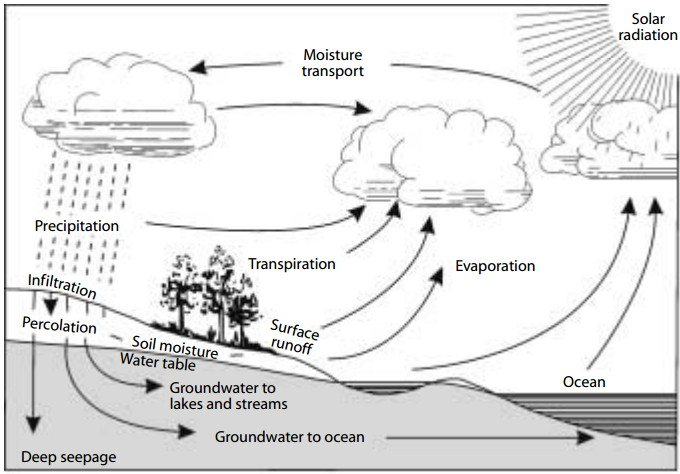
\includegraphics[width=.85\linewidth]{gfx/hydrocycle}
\end{center}
\caption{The hydrological cycle\citep{Zhang2002}. Reprinted from ``Water balance modelling: concepts and applications'', by \citeauthor{Zhang2002}, 2007, \emph{ACIAR MONOGRAPH SERIES, 84}, p.33. Copyright 2002 by \citeauthor{Zhang2002}.  }
\label{fig:hydrocycle}
\end{figure}
\newline
A variety of water balance models that are derived from \autoref{eq:generalwaterbalance} exists, it can have different levels of complexity depending on the objectives of the study and data availability. 
\section{Simple bucket model}
Simple bucket model is a widely-used water balance model in a simple conceptual scenario. It considers the controlled volume system as a bucket which is filled up from rainfall and emptied by evapotranspiration. If the bucket is full, extra water added is considered deep drainage. The only data that are necessary for this model are precipitation, evaporation, transpiration and the water storage capacity of the volume. 
\section{Root zone water balance}
 The water balance model can also be applied in relatively small scaled field studies based on a specific root zone soil water balance equation \citep{Ma2013}, given as:
\begin{align}
(\theta_t - \theta_{t-1})H &= P+I-D-ET-R\label{eq:rootzonewaterbalance}
\end{align}
\begin{quote}
Where \\
$\theta_t$ and $\theta_{t-1}$ are the initial and final depth-averaged soil water content of the root zone in one time step. \\
$H$ is the root zone depth.\\
$P$ is the precipitation.\\
$I$ is the Irrigation.\\
$D$ is the drainage out of the root zone, the positive value of D means downward percolation out of the root zone, whereas the negative value of it indicates upward capillary rise into the root zone.\\ $ET$ is the actual evapotranspiration.\\
$R$ is the surface runoff. 
\end{quote}
\autoref{fig:catchment} shows the relation of a root zone modelled by the root zone water balance \autoref{eq:rootzonewaterbalance} as a plot-sized profile in a catchment. The catchment can be considered as a collection of such root zone profiles, of which the total recharge in the catchment is estimated by adding the recharge from each profile. \\
\begin{figure}[bth]
\begin{center}
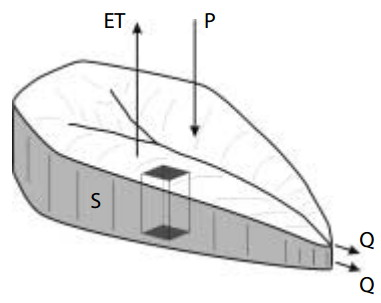
\includegraphics[width=0.5\linewidth]{gfx/catchment}
\caption{Schematic diagram of a catchment\citep{Zhang2002}. The box indicates the control volume of a root zone. S is water balance, ET is evapotranspiration, P is precipitation, Q is water runoff or flow. Reprinted from ``Water balance modelling: concepts and applications'', by \citeauthor{Zhang2002}, 2007, \emph{ACIAR MONOGRAPH SERIES, 84}, p.36. Copyright 2002 by \citeauthor{Zhang2002}. }\label{fig:catchment}
\end{center}
\end{figure}
\newline
This generalisation from root zone model is not applicable to catchments that contain complex lateral redistribution of water, thus it is difficult to estimate the recharge at a catchment scale. In most cases, it is inappropriate to assume that the catchment-scale recharge is equal to the sum of plot-scale water balance recharges, without in-depth research of the hydrogeological condition of the catchment, such as the recharge pathways and spatial heterogeneity of soil properties\citep{Zhang2002}.
 
\section{Complex models}
There are complex models that investigate not only the soil moisture dynamics but also the overall hydrological cycle over a large region of interest, they are designed to simulate interactions of different components within the system and to provide more thorough experimental results of many aspects\citep{Zhang2001}. For some purposes, simple bucket water balance models are appropriate, but other uses require greater functionality and/or more extensive analysis on a large geographic scale. For example, when analyzing the ecosystem of a large area of interest, there are various feedback between processes and different sub-systems that need to be taken into account, including the hydrological cycle, nutrient balance of soil and vegetation, heat balance, atmospheric change and more.
\subsection{Example: Study of Amazon Basin- a system in equilibrium}
For instance, the Water Balance Model can be applied to the entire Amazon Basin in Brazil, South America  \citep{Salati1984a}, which explains the status of water flow in the Amazon forest ecosystem in a quantitative manner, as shown in \autoref{fig:amazonWaterBalance}. \\
\begin{figure}[bth]
\begin{center}
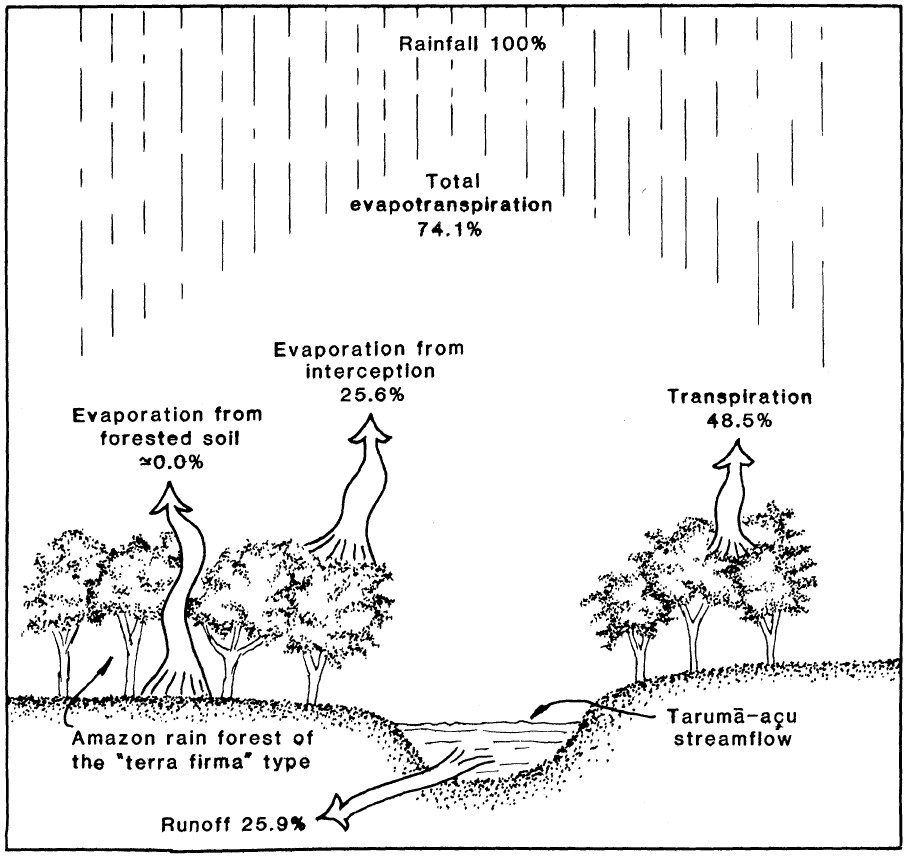
\includegraphics[width=.75\linewidth]{gfx/amazonWaterBalance}
\end{center}
\caption{Water balance from a study of a model basin near Manaus, Brazil\citep{Leopoldo1982}. Reprinted from ``Amazon basin: a system in equilibrium'', by \citeauthor{Salati1984a}, 1984, \emph{Science,4658}, p.130. Copyright 1984 by \citeauthor{Salati1984a}.  }
\label{fig:amazonWaterBalance}
\end{figure}
\newline
This model applies to the horseshoe-shaped Amazon Basin as a whole system, it uses knowledge of different domains in meteorology. However, due to the lack of proper infrastructure in Brazil when the study was conducted, accurate measurements on precipitation, evapotranspiration and other hydrological attributes over a large area were not available for analysis at a high precision level. \\
\newline
The measurements were taken from 1981 to 1983 in a controlled field in Barro-Branco watershed\citep{Leopoldo1995}. Precipitation data was obtained by use of a simple rain gauge installed at the reserve's meteorological station whereas the discharge was determined by use of a 0.8-m-wide rectangular weir and a water level recorder. Thus, the inferences of the influx and efflux of water in the area are based on assumptions made from wind conditions and a single point-based data as the averaged value over large areas which includes non-forest areas and are also influenced by other factors. 

\section{Water Balance Model of the Thesis}\label{section:waterbalancethesis}
There is a trade-off in choosing between complex models and simpler models such as the simple bucket model for conducting the analysis in this thesis. With greater functionality comes greater complexity. One of the issues with using a more complex water balance model is that there are more parameters required to complete the model. Which means that more data and man-hours are involved to understand and interpret the equation into a machine-readable form. If there isn't sufficient data of various parameters, then selecting a complex model is inappropriate for the objectives. The key to successful modelling is to match model complexity with data availability and the analysis objectives.
\subsection{Data availability}\label{subsection:dataavailability}
The objective of analysis in this thesis primarily concentrates on Australia as opposed to any other regions. Thus, one of the main data source being used is the \ac{awap}, which provides historic temporal-spatial meteorology data for the entire Australia. As described in the AWAP Final Report \citep{Raupach2009}, the AWAP is a partnership between \ac{cmar}, the \ac{bom} and the \ac{brs}, aiming to monitor the status and trend of the water balance of the Australian territories, using model-data fusion methods to combine measurements and model predictions. The AWAP data is discussed in more detail in \autoref{ch:dataintegration} \nameref{ch:dataintegration}.\\
\newline
The AWAP provides essential meteorology data for water balance calculations, such as the precipitation, evapotranspiration, surface runoff and deep drainage etc.\\
\newline
A farm location in Richmond, Tasmania, Australia, of geographic coordinate latitude: -42.61 and longitude: 147.39, is chosen for demonstration purpose. The location is marked on Google Maps\citep{Google2014} as shown in \autoref{fig:gmapexample}.\\
\begin{figure}[hbt]
\begin{center}
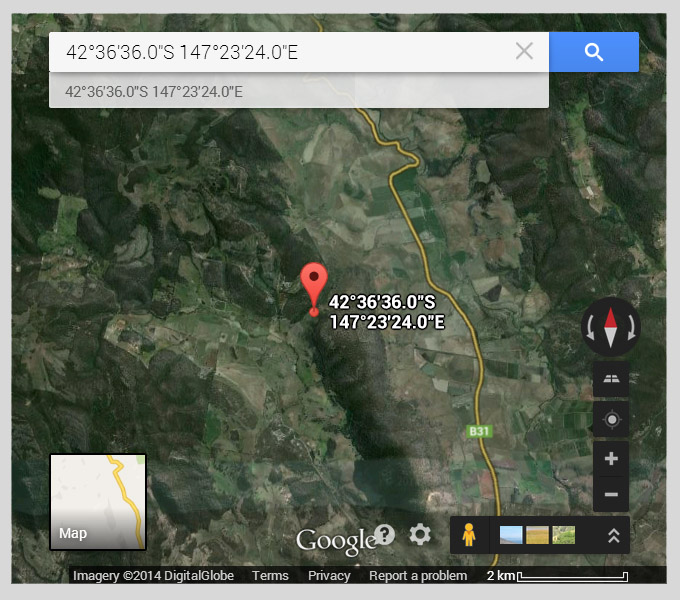
\includegraphics[width=0.75\linewidth]{gfx/gmapexample}
\end{center}
\caption{Satellite View of location latitude: -42.61 and longitude: 147.39, in Tasmania, Australia. Acquired from Google Maps.}
\label{fig:gmapexample}
\end{figure}
\newline
For this given location, the following time-series data of meteorology attributes: precipitation, evapotranspiration of soil and vegetation, open water evapotranspiration, surface runoff and deep drainage are acquired from AWAP, plotted in \autoref{fig:raints}, \autoref{fig:evapts}, \autoref{fig:surfrunts} and \autoref{fig:deepdraints} respectively. \\
\begin{figure}[hbt]
\begin{center}
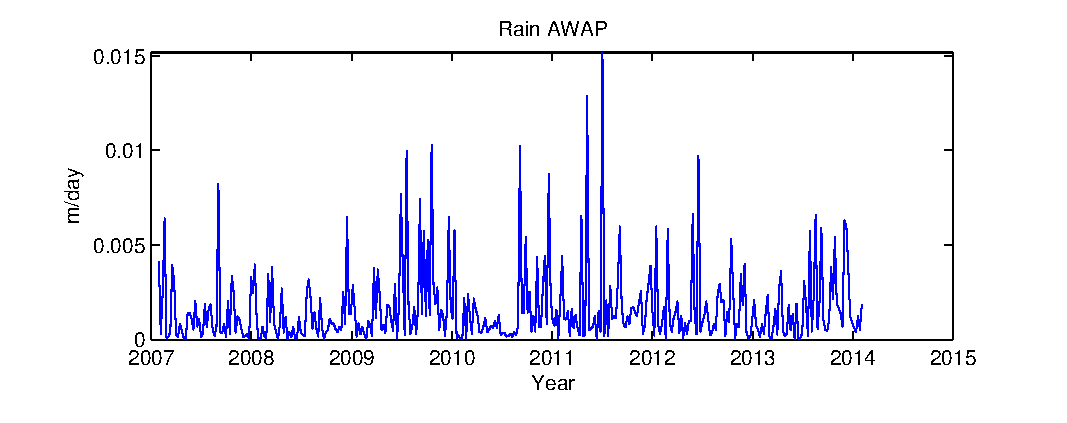
\includegraphics[width=\linewidth]{gfx/raints.eps}
\end{center}
\caption{Time series of AWAP data: Rainfall, for location lat: -42.61, lon:147.39}
\label{fig:raints}
\end{figure}
\newline
\autoref{fig:raints} shows the rainfall data of this location, plotted from Year 2007 to 2014. It has shown a consistent amount of precipitation for each of the years. The maximum rainfall per day is 0.0152 m/day which occurred during the week of 04-Jul-2011. Furthermore, year 2011-2012 has a slightly higher overall precipitation amount than the other years. In general, the chosen location has a dry start, then wet in Summer and Autumn throughout the year\citep{tasmania2013}. \\
\begin{figure}[hbt]
\begin{center}
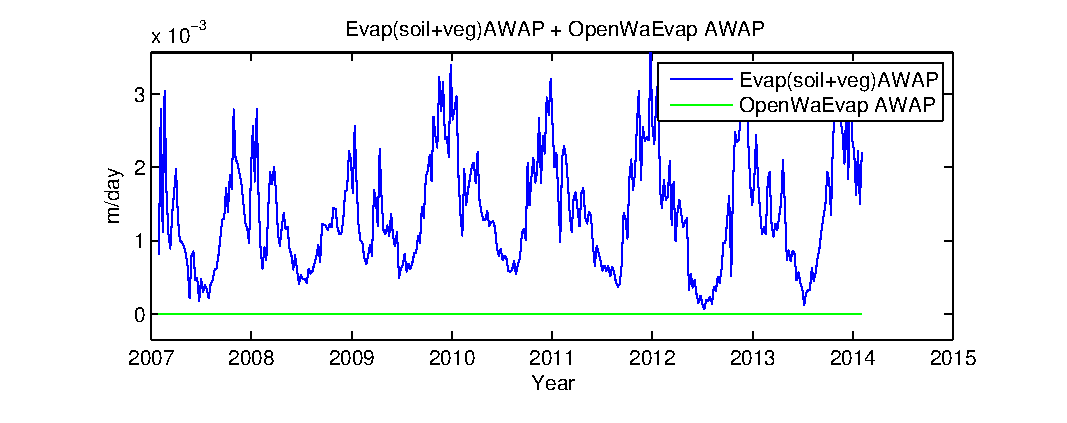
\includegraphics[width=\linewidth]{gfx/evapts.eps}
\end{center}
\caption{Time series of AWAP data: Evapotranspiration of soil and vegetation, and Open water evapotranspiration, for location lat: -42.61, lon:147.39}
\label{fig:evapts}
\end{figure}
\newline
\autoref{fig:evapts} shows the evapotranspiration data of this location. The blue line indicates the combined evapotranspiration of soil and vegetation, which has a clear and consistent chronological pattern throughout the years. The evapotranspiration reaches its lowest point during Winter season and climbs up to the highest point in the Summer season, which then declines during Autumn thus forming a repetition pattern. \\
On the other hand, open water evapotranspiration is indicated by the green line, which remains as zero for this location, due to the lack of open water in the surrounding terrestrial environment.\\
\begin{figure}[hbt]
\begin{center}
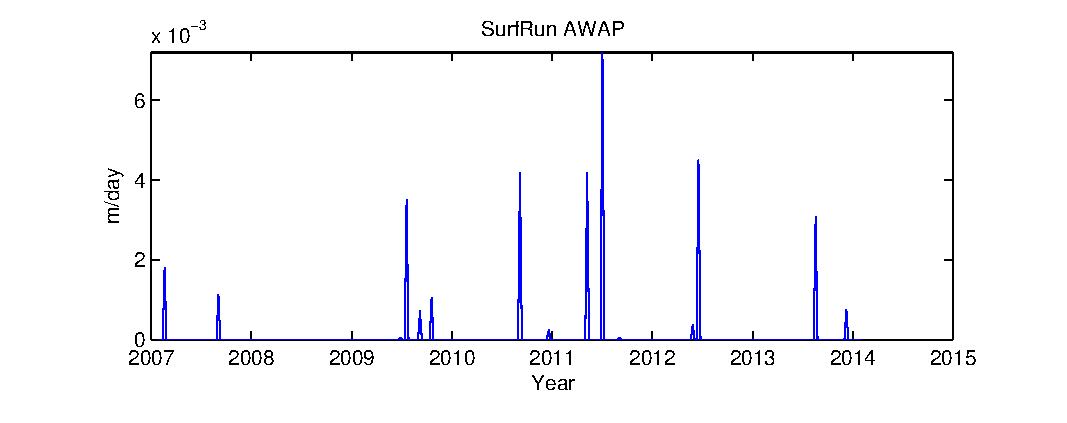
\includegraphics[width=\linewidth]{gfx/surfrunts.eps}
\end{center}
\caption{Time series of AWAP data: Surface Runoff, for location lat: -42.61, lon:147.39}
\label{fig:surfrunts}
\end{figure}
\newline
\autoref{fig:surfrunts} shows the surface runoff data of this location. Throughout the timespan, most of the weeks' surface runoff are zero while there are a few spikes in the figure. According to the AWAP datasheet\citep{Raupach2009}:
\begin{quote}
\emph{Surface runoff (FWRun) is given by a step function: all precipitation runs off when the upper-layer soil is saturated, and there is no runoff otherwise.}
\end{quote}
\begin{figure}[hbt]
\begin{center}
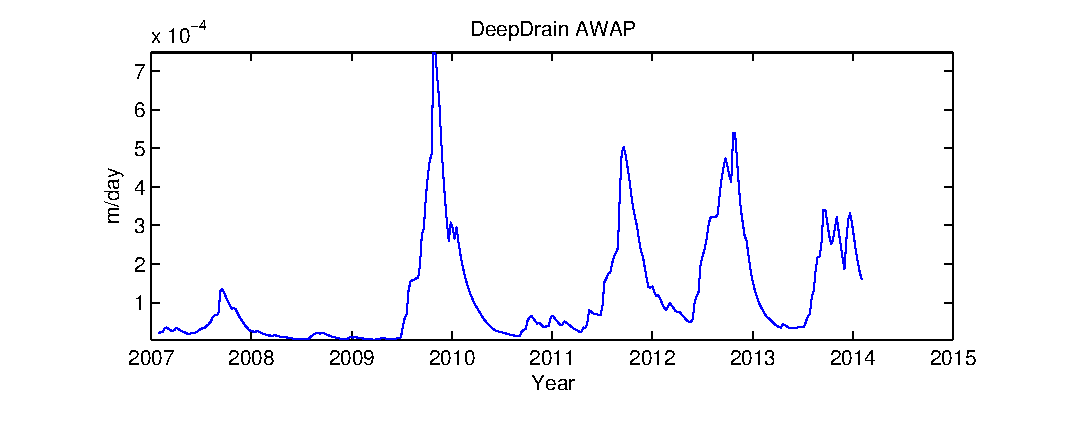
\includegraphics[width=\linewidth]{gfx/deepdraints.eps}
\end{center}
\caption{Time series of AWAP data: Deep Drainage, for location lat: -42.61, lon:147.39}
\label{fig:deepdraints}
\end{figure}
\begin{figure}[hbt] 
\begin{center}
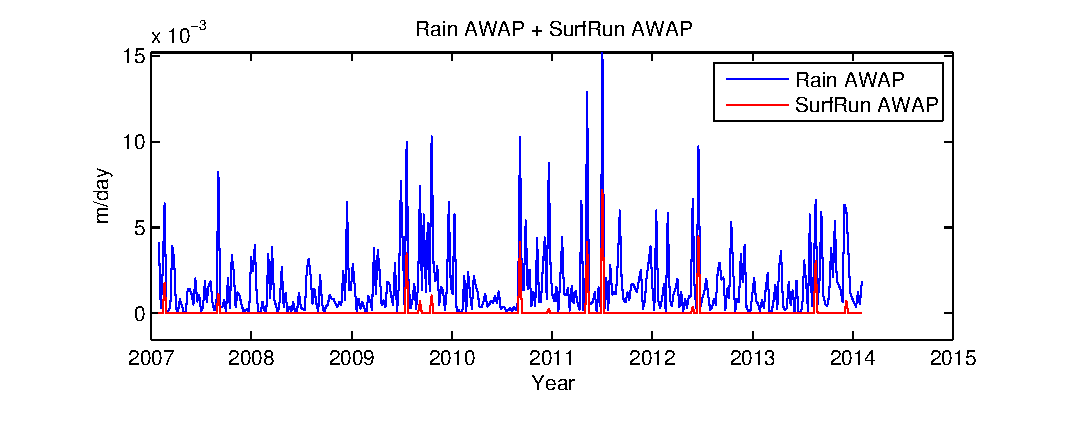
\includegraphics[width=\linewidth]{gfx/rainsurfts.eps}
\end{center}
\caption{Time series of AWAP data: Rainfall and Surface Runoff, for location lat: -42.61, lon:147.39}
\label{fig:rainsurfts}
\end{figure}
As shown in \autoref{fig:rainsurfts}, by comparing the rainfall data, as indicated by the blue line, and the surface runoff data, as indicated by the red line, we can confirm that the above statement is correct, because the spikes of surface runoff only occur where there are continuously heavier rainfalls. That is, surface water runoff occur only when the soil moisture is in saturation status due to heavy and continuous precipitation.\\
\newline
\autoref{fig:deepdraints} shows the deep drainage data of this location. By observing the curve itself, there is not any linear or chronological pattern apparent in the data. Nevertheless, according to the AWAP datasheet:
\begin{quote}\begin{minipage}{0.9\textwidth}
\emph{Leaching ($F_{\text{WLch}}$) or drainage downward out of soil layer i is given by}
\begin{align}
F_{\text{WLch}~i} &= K_{Si}w_i^\gamma
\label{eq:awapleaching}
\end{align}
\emph{Where $\gamma$ is an exponent specifying the response of drainage to relative soil water $w_i$, and $K_{Si}$ [m/day] is the saturated hydraulic conductivity of soil layer i.}
\end{minipage}\end{quote}
\begin{figure}[hbt]
\begin{center}
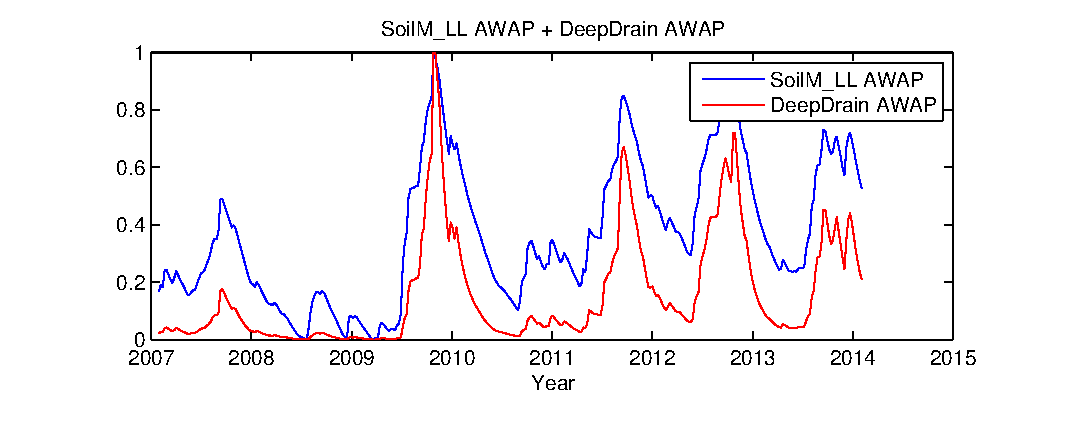
\includegraphics[width=\linewidth]{gfx/soilmdeepts.eps}
\end{center}
\caption{Time series of normalized AWAP data: Deep Drainage and Soil Moisture of low level, for location lat: -42.61, lon:147.39}
\label{fig:soilmdeepts}
\end{figure}
\autoref{fig:soilmdeepts} plots the soil moisture of low level and normalized deep drainage on the same figure. The data are normalized against the minimum and maximum so that both data scale from 0 to 1. There is an apparent direct correlation between the two meteorological attributes of the point of interest, which confirms the relationship defined in \autoref{eq:awapleaching}. This means that deep drainage occur if the lower level of soil moisture is saturated.
\subsection{Implementing water balance model}\label{subsection:implementwaterbalance}
In this thesis, a water balance model is implemented from the equation 
\begin{align}
	\Delta \langle S\rangle &= \langle P\rangle - \langle ET\rangle-\langle Q\rangle-\langle R\rangle
	\label{eq:wbsimple}
\end{align}
\begin{quote}Where \\
\indent$\Delta \langle S\rangle$ is the change in spatially averaged catchment water storage, which ideally is zero when there is perfect balanced influx and efflux of the system.\\
\indent$\langle P\rangle$ is the spatially averaged precipitation, acquired from AWAP rainfall data, represented by the variable \emph{\{rain AWAP\}} in the integrated data source.\\
\indent$\langle ET\rangle$ is the spatially averaged catchment evapotranspiration, acquired by adding two variables from AWAP, evapotranspiration of soil and vegetation \& open water evapotranspiration, represented in the integrated data source as \emph{\{Evap(soil+veg)AWAP + OpenWaEvap AWAP\}}.\\
\indent$\langle Q\rangle$ is the spatially averaged catchment surface runoff, acquired from AWAP surface runoff data, represented by the variable \emph{\{SurfRun AWAP\}}.\\
\indent$\langle R\rangle$ is the spatially averaged catchment recharge, acquired from AWAP deep drainage data, represented by the variable \emph{\{DeepDrain AWAP\}}, while sub-surface flow is considered zero.
\end{quote}
\begin{figure}[hbt]
\begin{center}
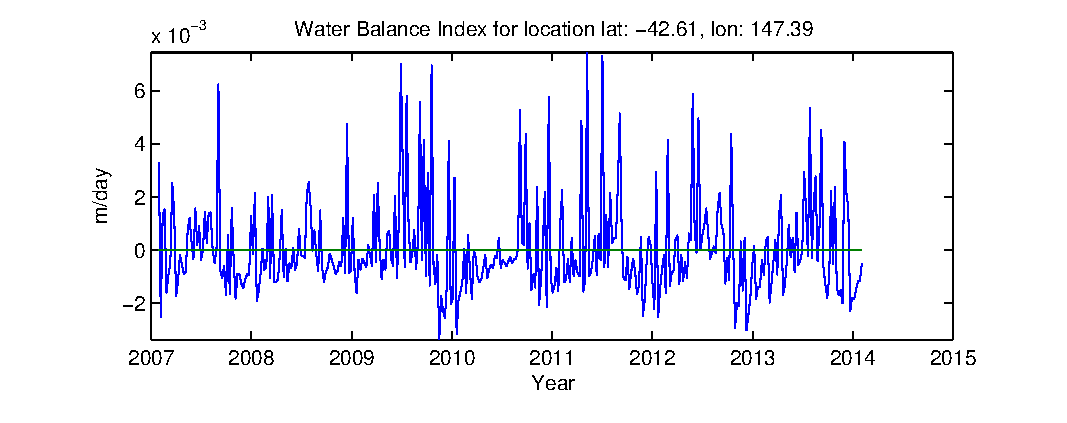
\includegraphics[width=\linewidth]{gfx/waterts.eps}
\end{center}
\caption{Time series of calculated water balance index from AWAP data, for location lat: -42.61 lon:147.39}
\label{fig:waterts}
\end{figure}
\autoref{fig:waterts} plots the calculated water balance index for the given location from year 2007 to 2014, using \autoref{eq:wbsimple}. For this point of interest, the water balance index fluctuates around the zero line, which means during the time when there is rainfall, the water balance is at higher level, and vice versa.\\
\begin{figure}[hbt]
\begin{center}
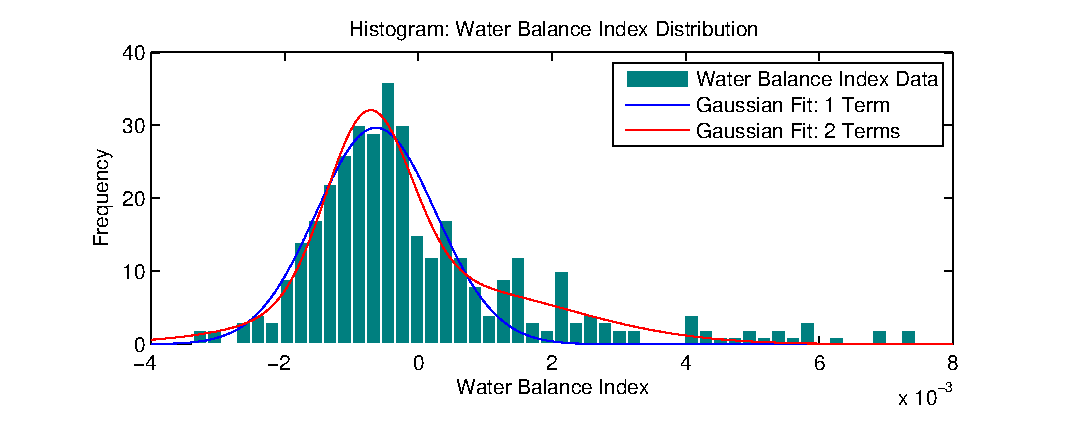
\includegraphics[width=\linewidth]{gfx/waterhist.eps}
\end{center}
\caption{Histogram of calculated water balance index with fitted Gaussian Distribution}
\label{fig:waterhist}
\end{figure}
\newline
The histogram of the water balance index data is plotted with 50 bars, as shown in \autoref{fig:waterhist}. Two Gaussian distributions are generated to fit the data, both one term and two terms fittings, the parameters are given below.
\begin{quote}
\begin{align}
f(x)&=a_1*e^{-((x-b_1)/c_1)^2)}\label{eq:gaussianfit1}\\
g(x)&=a_2*e^{-((x-b_2)/c_2)^2)}+a_3*e^{-((x-b_2)/c_2)^2)}
\end{align}
Where the coefficients (with 95\% confidence bounds) are:\\
$a_1 = 29.68~(26.58, 32.78)\\
b_1 =  -0.0006337~ (-0.0007418, -0.0005256)\\
c_1 =    0.001269  ~(0.001116, 0.001422)\\
a_2 =       25.25 ~ (20.61, 29.89)\\
       b_2 =  -0.0007439 ~ (-0.0008451, -0.0006426)\\
       c_2 =   0.0008972  ~(0.000711, 0.001083)\\
       a_3 =       7.916  ~(4.042, 11.79)\\
       b_3 =   0.0003042~  (-0.00053, 0.001138)\\
       c_3 =    0.002693  ~(0.001877, 0.00351)$
\end{quote}
From the Gaussian distribution fittings in \autoref{fig:waterhist}, the data generally is normally distributed while slightly skewed to the right. This indicates that water balance index like most meteorological attributes which naturally has a centralising tendency and certain variations due to fluctuations in the surrounding environment and/or seasonal changes, thus it can be used as a good indication for irrigation water usage.
